\documentclass[a4paper,final]{memoir}

% Language and encoding
\usepackage[utf8]{inputenc}
\usepackage[T1]{fontenc}
\usepackage[english]{babel}
\usepackage[protrusion=true,expansion=true]{microtype} % better typography

% Math
\usepackage{amsmath,amssymb,amsfonts,amsthm,latexsym}


\newtheorem{thm}{Theorem}[chapter]
\theoremstyle{definition}

%\newtheoremstyle{mydefstyle}
%  {3\topsep} % Space above
%  {3\topsep} % Space below
%  {} % Body font
%  {} % Indent amount
%  {\bfseries} % Theorem head font
%  {} % Punctuation after theorem head
%  {.5em} % Space after theorem head
%  {} % Theorem head spec (can be left empty, meaning `normal')
%
%\theoremstyle{mydefstyle}
\newtheorem{defn}{Definition}[chapter]
%\newtheorem{examp}[thm]{Example}

\newcommand{\bbN}{\mathbb N} %the natural numbers
\newcommand{\bbZ}{\mathbb Z} %the integers
\newcommand{\bbQ}{\mathbb Q} %the rational numbers
\newcommand{\bbR}{\mathbb R} %the real numbers
\newcommand{\bbC}{\mathbb C} %the complex numbers

%\providecommand*{\listingautorefname}{Listing}

% Graphic stuff
\usepackage[pdftex]{graphicx}
\usepackage[usenames,dvipsnames,table]{xcolor}
\definecolor{shade}{RGB}{245,245,245}
\usepackage[pdftex,colorlinks=true]{hyperref}
\hypersetup
{
    bookmarksnumbered,
    linkcolor=RoyalBlue,
    anchorcolor=RoyalBlue,
    citecolor=RoyalBlue,
    urlcolor=RoyalBlue,
    pdfstartview={FitV},
    pdfdisplaydoctitle
}
\usepackage{pgfplots}

% Tables
\usepackage{booktabs}
\usepackage[hang,small,bf]{caption}

% Debug, etc.
\usepackage{todonotes}

% Numbering
\setsecnumdepth{subsection}
\maxtocdepth{subsection}
\numberwithin{equation}{chapter}
\numberwithin{figure}{chapter}
\numberwithin{table}{chapter}

% Computer science stuff
\usepackage{clrscode3e}
\usepackage{verbatim}
\newcommand{\mono}[1]{{\ttfamily#1}}
\usepackage{listings}
\lstset
{
    tabsize=2,
    numbers=left,
    breaklines=true,
    backgroundcolor=\color{shade},
    framexleftmargin=0.05in,
    basicstyle=\ttfamily\small,
    numberstyle=\tiny,
    keywordstyle=\color{RoyalBlue},
    stringstyle=\color{Maroon},
    commentstyle=\color{ForestGreen}
}


% Document meta stuff
\newcommand{\horrule}[1]{\rule{\linewidth}{#1}}
\makeevenfoot{plain}{}{}{\thepage}
\makeoddfoot{plain}{}{}{\thepage}

\begin{document}

\frontmatter

\begin{titlingpage}
\begin{center}

\usefont{OT1}{bch}{b}{n}
\normalfont \normalsize
\textsc{Department of Computer Science, University of Copenhagen} \\ [25pt]
\horrule{0.5pt} \\ [0.4cm]
\huge Estimated stretch of Approximate Distance Oracles \\
\horrule{2pt} \\ [0.5cm]
\normalfont \normalsize
Bachelor project by \\ \normalsize
Jonas Brunsgaard \\ \normalsize
\mono{jonas.brunsgaard@gmail.com} \\ [+6pt] \normalsize
Supervisor: Mikkel Thorup \\ [+6pt] \normalsize
\today

\end{center}
\end{titlingpage}

%\thispagestyle{empty}

\begin{abstract}
Approximate distance oracle is a data structure presented by Thorup and
Zwick\cite{tu} that allows for approximate shortest path queries in
constant time on undirected connected graphs with positive edge weights.
The approximated distances is said to be of \emph{Stretch-3}, if the data
structure is constructed in such a way that the produced estimates, is at most
a factor three longer than the actual shortest path.

In this report I look at the actual stretches produces by \emph{Stretch-3}
approximate distance oracles. Through experiments I attempt to indicate
a value of the expected actual stretch, in graphs representing internet
topologies and road networks. To perform the experiments, a high performance
C++ implementation of approximate distance oracles has been developed and is
discussed in the report.

Based on experiments over internet topologies from Stanford Large Network
Data\cite{snapnets} collection. I find that the tested graphs on average produce stretches
of $\sim1.5$. When conducting the experiments over road networks from California,
Texas and Pennsylvania the average actual stretch is $\sim1.1$. I find the graphs
of each domain to produce very similar results and the distribution of the
actual stretches produced is also a like.

Thus I find these values to be reasonable indicators for the average actual
stretch for their domains.
\end{abstract}


\newpage
\tableofcontents

\pagestyle{Ruled}
\chapterstyle{hangnum}
\mainmatter

\newpage
\chapter{Introduction}
\label{sec:introduction}

Finding the shortest path between a vertex pair in a graph is one
of the most fundamental computational graph problems. Papers like
Dijkstra\cite{Dijkstra59anote} and Bellman-Ford\cite{bellman} presents
algorithms able to determine the shortest path for a single vertex pair, but
these algorithms does not scale well, as they need to visit every vertex in
the graph to come up with a result. Thus, these algorithms are a poor choice
for applications that needs to answer shortest path queries for large graphs
extremely fast.

Now suppose you are given a connected weighted undirected graph $G=(V,E)$
consisting of $n$ vertices and $m$ edges, and you are asked to come up with a
solution able to answer shortest path queries extremely fast.

The naive solution is to compute the shortest path between every vertex pair
$(u,v) \in V \times V$ and store the information in a lookup table using
$(u,v)$ as key for the entry. Subsequent distance queries can be answered in
constant time simply by performing a lookup in the hash table.
However, there are strong objections to this naive solution.

First of all the preprocessing time may simply be too long, and secondly,
even if one is willing to wait for the preprocessing to finish, the size of
the final lookup table may be too large to store efficiently. Using Thorups
shortest path algorithm for undirected graphs\cite{thorupsssp}, which offers
$O(m)$ time complexity, to compute the distances from each vertex $v\in V$,
one gets a time complexity of $O(nm)$ while $O(n^2)$ space is required by the
lookup table.

If one can settle for approximated distances instead of exact ones,
approximate distance oracles is the better alternative for undirected
graphs. Approximate distance oracles is a data structure presented by Thorup
and Zwick\cite{tu}, it offers much better space and construction time
complexities, while still being able to answer shortest path queries in
constant time.

More precisely the paper describe for any integer $k \leq 1$, a preprocessing
algorithm that runs $O(kmn^{1/k})$, producing a data structure of size
$O(kn^{1+1/k})$. The data structure can return approximate distances of a
finite stretch $t$. An estimated distance $\hat{\delta}(u,v)$ from $u$ to $v$
is said to be within the stretch $t$ if and only if $\delta(u,v)\leq
\hat{\delta}(u,v)\leq t \cdot\delta(u,v)$ where $\delta(u,v)$ denotes the
exact shortest distance. The actual stretch of the produced estimates is
at most $2k-1$, but it may be as low as $1$. Thorup and Zwick does not discuss
this further.

In this report I study - through experiments - the average actual stretch of
distances produced by \emph{Stretch-3} ($k=2$) approximate distance oracles. A
high quality implementation of the algorithm has been developed to conduct
the experiments, and has been used to compute approximate distance oracle
data structures for graphs representing internet topologies and road networks.

Using a sample of vertex pairs from each graph, and comparing the actual
shortest path against the approximated shortest path in the sample, I show the
average actual stretch for these internet topologies and road networks. The
goal is to provide data that indicates what actual stretch to expect, if you
apply approximate distance oracles to these classes of graphs.

The rest of the article is organized as follows: In the next short chapter I
introduce some basic background material. Then, \autoref{sec:ado} presents an
introduction to approximate distance oracles. In \autoref{sec:implementation}
I discuss obstacles and solution regarding the implementation and development
process. Finally in \autoref{sec:experiments} I conduct and discuss my
experiments before I present my conclusions in \autoref{sec:conclusion}.

\newpage
\chapter{Background material}

\section{The shortest path problem}
The shortest path problem is, as mentioned in the previous section, a well
known graph problem. Nevertheless I allow myself to brush up the readers
memory and define the problem.
\begin{defn}
    For a graph $G = (V, E)$ and a weight function $w : E \rightarrow
    \mathbb{R}$ mapping edges to edge weights.
    A path $p$ in $G$ is expressed by a sequence of vertices, where each
    vertex is adjacent with the next vertex in the sequence.
    \[
        p = \langle v_0, v_1, \dots ,v_i \rangle
    \]
    The weight of a path $w(p)$ is then given by the sum of the edge weights:
    \[
        w(p) = \sum\limits_{i=1}^k w(v_{i-1},v_{i})
    \]
    For two vertices $u,v \in V$. The \textbf{(shortest) distance}
    $\delta(u,v)$ from $u$ to $v$, is defined as:
    \[
        \delta(u,v) =
            \begin{cases}
                \text{min} \{ w(p): u \overset{p}{\leadsto} v \}
                & \text{if there exists a path from $u$ to $v$} \\
                \infty
                & \text{otherwise }
            \end{cases}
    \]
    A path $p$ from $u$ to $v$ is then a \textbf{shortest path} if and only if
    $w(p) = \delta(u,v)$.
\end{defn}
The shortest path problem described above may be referred to as \emph{single
pair shortest path}, but solutions to this problem requires the growth of
a shortest path tree from the source vertex, thus the computational
complexity of finding a shortest path between a vertex pair, is essentially the
same as finding the shortest path from the source vertex to all other vertices
in the graph.
Therefore the problem is often just referred to as \emph{single source
shortest path} or SSSP, even though in many cases only the distance
between a single vertex pair is of interest.

When constructing the approximate distance oracle data structure SSSP is
computed multiple times, thus in production environments an efficient SSSP
algorithm is needed. As mentioned in the previous section Thorup has presented
a SSSP algorithm for undirected graphs that offers a running time of $O(m)$
\cite{thorupsssp}. In the rest of this report I assume that SSSP is solved in
$O(m)$ unless mentioned otherwise.

\section{Shortest distances in large graphs}
Recent years - as we enter the age of big data - larger and larger graphs are
emerging. The World Wide Web, social networks, navigation service applications
and more has brought new attention to the shortest path problem, due the
increased space and time consumed by these new large graphs. Efficient
algorithms for the shortest path problem are important for two main reasons.

First of all, shortest path queries are the core product of many graph
applications, such as Google Maps, where a user requests a shortest path
between e.g Aarhus and Copenhagen.
Second, shortest path queries are used as building blocks in other algorithms
used to perform analytical tasks in graphs. E.g. centrality is calculated by
shortest path queries and include identifying the most influential persons in
a social network, key infrastructure nodes in the Internet, etc.
Also other measures, such as network diameter and betweenness, are based on
shortest path queries.

Well known algorithms such as Dijkstra and Bellman Ford solves the
problem of finding a shortest path, but a noticeable drawback of these
algorithms is that they are too slow for applications were fast results
are essential. The article "Toward a Distance Oracle for Billion-Node
Graphs"\cite{sp_billion_nodes} claim that for graphs of "web scale" it takes
hours for the Dijkstra algorithm to terminate.

As mentioned in the Introduction, a naive attempt to improve the query
time of shortest paths is to pre compute the distances. But the $O(n^2)$
space consumption makes this solution rather unrealistic. To put this into
perspective the largest graph for which I run experiments has 2 million
vertices.

\autoref{fig:matrixgrowth} shows the relationship between number of vertices
in the graph and the space consumption for the entries, I assume that an
integer takes up 32 bit of storage. To create a lookup table for the graph
with 2 million vertices I would have to store 30 terabyte of data, which seems
problematic. Graphs of this size is far from unusual today.

\begin{figure}[htbp]
    \centering
    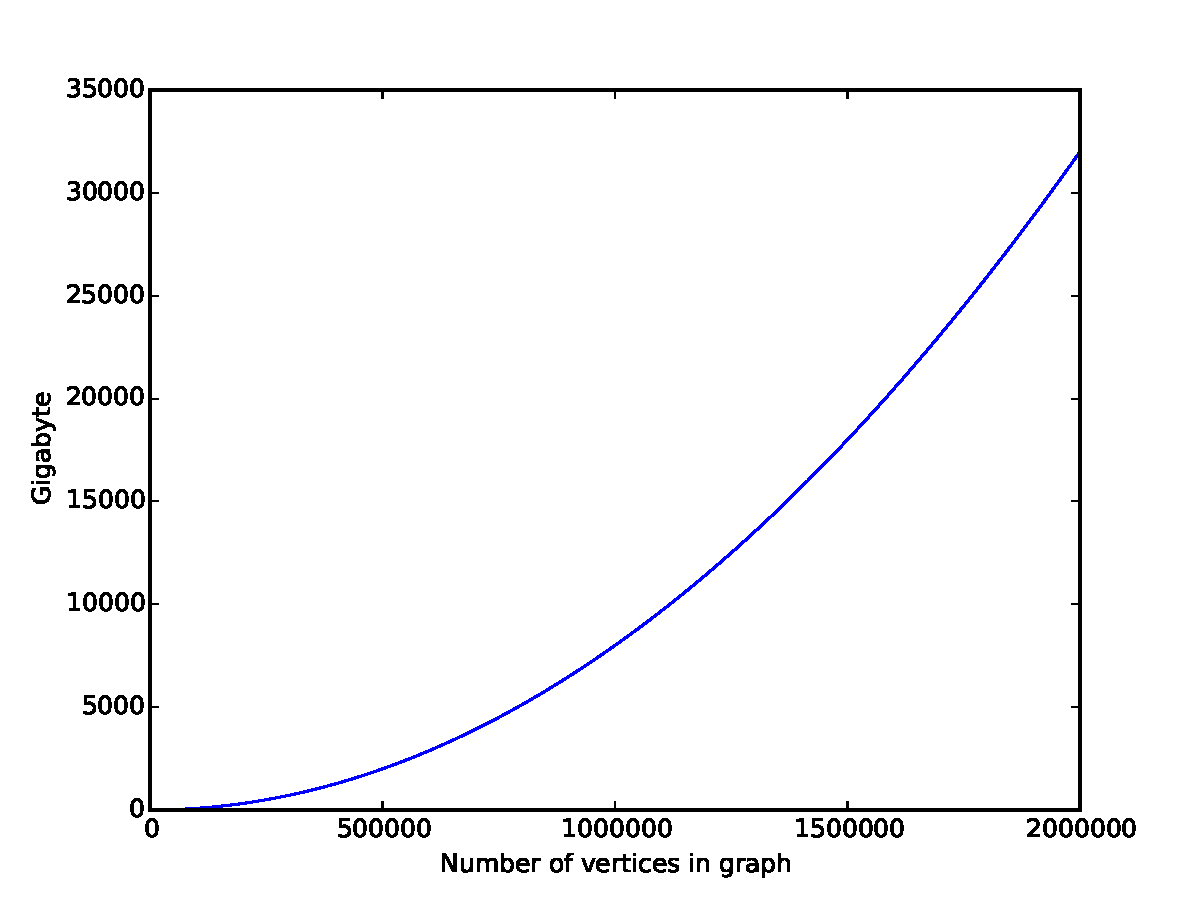
\includegraphics[width=\textwidth]{matrixsize.pdf}
    \caption{Space consumption for $n\times n$ matrix, with 32 bit integers as entries}
    \label{fig:matrixgrowth}
\end{figure}

In general there is no doubt that the naive approach is unrealistic, as space
consumption rapidly exceeds the amount of disk space and memory available in
most computing environments.

The growth in applications using shortest paths and growth in the size of
large graphs, has led to increased research in data structures, which are
still able to answer shortest path queries extremely fast, but with improved
space complexity. Approximate distance oracles is a result of this research.

\chapter{Approximate distance oracles}
\label{sec:ado}
Thorup and Zwick presents a in the A\&C seminal paper "Approximate Distance
Oracles"\cite{tu}, the construction of a data structure that subsequently
can be used to answer shortest path queries extremely fast. The method can
be applied to connected undirected graphs with positive edge weights and is
feasible where approximated results are acceptable.

The paper sets forward two algorithms. The first one is the algorithm for
constructing the data structure called, we will refer to this algorithm as
\proc{propro}. The second one we call \proc{dist} and is used for querying
the data structured.

\proc{prepro} makes use of an integer $k$, that lets one weigh the precision
(maximum stretch) of the estimated distances versus space and time consumption.

An estimate of the shortest distance, denoted $\hat{\delta}$, from vertex $u$
to vertex $v$ is said to be of stretch $t$ if and only if
\begin{equation}
    \delta(u,v) \leq \hat{\delta}(u,v) \leq t \cdot \delta(u,v)
    \label{eq:stretchinterval}
\end{equation}
The properties of the data structure and the relationship between $k$ and the
stretch is formulated in the theorem below\footnote{\cite{tu}, Theorem 1.1}.
\begin{thm}
    Let $G=(V,E)$ be a weighed undirected graph with nonnegative edge weights
    with $|V|=n, |E|=m$. Let $k \geq 1$ be an integer. Then, the graph $G$
    can be preprocessed in $O(kmn^{1/k})$ expected time, producing a data
    structure of $O(kn^{1+1/k}$, such that subsequent distance queries can
    be answered, approximately, in $O(k)$ time. The stretch of the produced
    estimates is at most $2k-1$. Paths no longer than the estimates returned
    can be produced in constant time.\footnote{In this report I do not care
    for the actual path found by the algorithm, only for the distance of
    the path, and thus the last sentence of Threorem\autoref{thm:ado_prop} is
    only present for completion.}
    \label{thm:ado_prop}
\end{thm}
By choosing $k=1$ we get a solution similar to computing all distances
and saving the results, that is $O(mn)$ preprocessing time, $O(n^2)$ space
consumption and a worst case stretch of $1$. When $k=2$ we get a
preprocessing time of $O(mn^{1/2})$, space consumption is $O(n^{3/2})$ and
the stretch is now $3$. This trend continues until $k \gets log(n)$. For $k$
greater than $log(n)$ space and time consumption will not improve as the
functions for space and time complexity finds their local minimum where $k
\gets log(n)$.

The essence of approximate distance oracles is to make use of a collection of
induced trees that form a tree cover of the whole graph. The reduced space
consumption is achieved, because each vertex is only contained in a small
number of the trees. The construction algorithm assures that for each vertex
pair there exists a tree with a small-stretched path between the two vertices.

From the trees the article derive a bunch $B(v) | v \in V$ for each vertex in
the graph. A bunch is a collection of vertices for which the shortest distance
is known. In practice a bunch $B(v)$ for a vertex $v$ is a hash map with a
vertex $u$ as key and the distance $\delta(u,v)$ as value.

Besides bunches, the algorithms make use what is referred to as witnesses.
A witness to a vertex $v$ is denoted as $p_{i}{v}$, where $i$ refers a
specific set ($A_{i}$) of vertices in the graph. The witness for a specific
vertex $v$ and set $A_{i}$ is a tuple containing a vertex $w$ and a distance
$\delta(v,w)$. The witness is the vertex in the set $A_{i}$, with the shortest
distance to $v$.

A graphic representation of bunches and witnesses for $u$ and $v$ is depicted
in \autoref{fig:bunches}.
\begin{figure}[htbp]
    \centering
\begin{tikzpicture}
    \filldraw[fill=white, draw=black] (0.04,4.81) circle [radius=1.50mm];
    \filldraw[fill=white, draw=black] (0.07,4.19) circle [radius=1.50mm];
    \filldraw[fill=white, draw=black] (0.08,0.08) circle [radius=1.50mm];
    \filldraw[fill=white, draw=black] (0.1,2.49) circle [radius=1.50mm];
    \filldraw[fill=white, draw=black] (0.47,3.68) circle [radius=1.50mm];
    \filldraw[fill=white, draw=black] (0.64,0.53) circle [radius=1.50mm];
    \filldraw[fill=white, draw=black] (0.81,2.42) circle [radius=1.50mm];
    \filldraw[fill=white, draw=black] (0.95,4.62) circle [radius=1.50mm];
    \filldraw[fill=white, draw=black] (1.23,2.87) circle [radius=1.50mm];
    \filldraw[fill=white, draw=black] (1.75,1.83) circle [radius=1.50mm];
    \filldraw[fill=white, draw=black] (1.78,4.86) circle [radius=1.50mm];
    \filldraw[fill=white, draw=black] (1.91,0.81) circle [radius=1.50mm];
    \filldraw[fill=white, draw=black] (2.02,4.27) circle [radius=1.50mm];
    \filldraw[fill=white, draw=black] (2.36,3.5) circle [radius=1.50mm];
    \filldraw[fill=white, draw=black] (2.39,2.78) circle [radius=1.50mm];
    \filldraw[fill=white, draw=black] (2.49,1.9) circle [radius=1.50mm];
    \filldraw[fill=white, draw=black] (2.57,1.14) circle [radius=1.50mm];
    \filldraw[fill=white, draw=black] (2.57,4.83) circle [radius=1.50mm];
    \filldraw[fill=white, draw=black] (3.07,1.68) circle [radius=1.50mm];
    \filldraw[fill=white, draw=black] (3.09,4.02) circle [radius=1.50mm];
    \filldraw[fill=white, draw=black] (3.16,3.13) circle [radius=1.50mm];
    \filldraw[fill=white, draw=black] (3.2,4.96) circle [radius=1.50mm];
    \filldraw[fill=white, draw=black] (3.25,1.02) circle [radius=1.50mm];
    \filldraw[fill=white, draw=black] (3.84,3.36) circle [radius=1.50mm];
    \filldraw[fill=white, draw=black] (3.91,2.28) circle [radius=1.50mm];
    \filldraw[fill=white, draw=black] (4.41,1.45) circle [radius=1.50mm];
    \filldraw[fill=white, draw=black] (4.83,0.28) circle [radius=1.50mm];
    \filldraw[fill=white, draw=black] (5.22,1.86) circle [radius=1.50mm];
    \filldraw[fill=white, draw=black] (5.45,2.9) circle [radius=1.50mm];
    \filldraw[fill=white, draw=black] (5.45,3.52) circle [radius=1.50mm];
    \filldraw[fill=white, draw=black] (5.57,4.45) circle [radius=1.50mm];
    \filldraw[fill=white, draw=black] (6.08,0.33) circle [radius=1.50mm];
    \filldraw[fill=white, draw=black] (6.14,1.58) circle [radius=1.50mm];
    \filldraw[fill=white, draw=black] (6.24,4.14) circle [radius=1.50mm];
    \filldraw[fill=white, draw=black] (6.25,2.93) circle [radius=1.50mm];
    \filldraw[fill=white, draw=black] (6.69,4.83) circle [radius=1.50mm];
    \filldraw[fill=white, draw=black] (6.88,1.6) circle [radius=1.50mm];
    \filldraw[fill=white, draw=black] (6.89,3.09) circle [radius=1.50mm];
    \filldraw[fill=white, draw=black] (7.13,0.95) circle [radius=1.50mm];
    \filldraw[fill=white, draw=black] (7.54,0.15) circle [radius=1.50mm];
    \filldraw[fill=white, draw=black] (7.89,3.09) circle [radius=1.50mm];
    \filldraw[fill=white, draw=black] (8.3,2.15) circle [radius=1.50mm];
    \filldraw[fill=white, draw=black] (8.46,1.41) circle [radius=1.50mm];
    \filldraw[fill=white, draw=black] (8.59,4.0) circle [radius=1.50mm];
    \filldraw[fill=white, draw=black] (8.74,0.53) circle [radius=1.50mm];
    \filldraw[fill=white, draw=black] (9.08,1.14) circle [radius=1.50mm];
    \filldraw[fill=white, draw=black] (9.12,3.34) circle [radius=1.50mm];
    \filldraw[fill=white, draw=black] (9.24,5.0) circle [radius=1.50mm];
    \filldraw[fill=white, draw=black] (9.3,4.29) circle [radius=1.50mm];
    \filldraw[fill=white, draw=black] (9.59,2.68) circle [radius=1.50mm];
    \filldraw[fill=white, draw=black] (9.67,0.58) circle [radius=1.50mm];
    \filldraw[fill=white, draw=black] (9.7,1.5) circle [radius=1.50mm];
    \filldraw[fill=white, draw=black] (9.96,0.04) circle [radius=1.50mm];
    \filldraw[fill=gray!50, draw=black] (0.04,1.34) circle [radius=1.50mm];
    \filldraw[fill=gray!50, draw=black] (0.66,1.31) circle [radius=1.50mm];
    \filldraw[fill=gray!50, draw=black] (1.4,3.46) circle [radius=1.50mm];
    \filldraw[fill=gray!50, draw=black] (1.74,2.52) circle [radius=1.50mm];
    \filldraw[fill=gray!50, draw=black] (3.89,0.59) circle [radius=1.50mm];
    \filldraw[fill=gray!50, draw=black] (4.49,3.85) circle [radius=1.50mm];
    \filldraw[fill=gray!50, draw=black] (4.57,3.11) circle [radius=1.50mm];
    \filldraw[fill=gray!50, draw=black] (4.69,4.69) circle [radius=1.50mm];
    \filldraw[fill=gray!50, draw=black] (4.92,2.5) circle [radius=1.50mm];
    \filldraw[fill=gray!50, draw=black] (5.02,1.18) circle [radius=1.50mm];
    \filldraw[fill=gray!50, draw=black] (5.4,0.69) circle [radius=1.50mm];
    \filldraw[fill=gray!50, draw=black] (6.85,4.07) circle [radius=1.50mm];
    \filldraw[fill=gray!50, draw=black] (7.55,4.29) circle [radius=1.50mm];
    \filldraw[fill=gray!50, draw=black] (7.76,1.61) circle [radius=1.50mm];
    \filldraw[fill=gray!50, draw=black] (8.15,0.14) circle [radius=1.50mm];
    \filldraw[fill=gray!50, draw=black] (8.66,2.71) circle [radius=1.50mm];
    \filldraw[fill=gray!50, draw=black] (9.99,3.56) circle [radius=1.50mm];
    \filldraw[fill=black!80, draw=black] (3,0.3) circle [radius=1.50mm];
    \filldraw[fill=black!80, draw=black] (4,4.7) circle [radius=1.50mm];
    \filldraw[fill=black!80, draw=black] (8.2,4.5) circle [radius=1.50mm];
    \filldraw[fill=white, draw=black] (3,2.5) circle [radius=1.50mm];
    \node at (3.3,2.3) {\small$v$};
    \draw(3,2.5) circle [radius=1.26015872016cm];
    \node at (1.4,2.22) {\small$p_1(v)$};
    \draw [->] (3,2.5) -- (1.74,2.52);
    \draw [->] (3,2.5) -- (3.07,1.68);
    \draw [->] (3,2.5) -- (2.36,3.5);
    \draw [->] (3,2.5) -- (2.39,2.78);
    \draw [->] (3,2.5) -- (3.91,2.28);
    \draw [->] (3,2.5) -- (2.49,1.9);
    \draw [->] (3,2.5) -- (3.16,3.13);
    \draw [->] (3,2.5) -- (3.84,3.36);
    \draw(3,2.5) circle [radius=2.2cm];
    \node at (3.6,0.2) {\small$p_2(v)$};
    \draw [->] (3,2.5) -- (1.74,2.52);
    \draw [->] (3,2.5) -- (3.89,0.59);
    \draw [->] (3,2.5) -- (4.49,3.85);
    \draw [->] (3,2.5) -- (1.4,3.46);
    \draw [->] (3,2.5) -- (4.57,3.11);
    \draw [->] (3,2.5) -- (4.92,2.5);
    \draw [->] (3,2.5) -- (4,4.7);
    \draw [->] (3,2.5) -- (3,0.3);
    \draw [->] (3,2.5) -- (8.2,4.5);
    \filldraw[fill=white, draw=black] (7,2.5) circle [radius=1.50mm];
    \node at (7.3,2.4) {\small$u$};
    \draw(7,2.5) circle [radius=1.17034183041cm];
    \node at (8.36,1.71) {\small$p_1(u)$};
    \draw [->] (7,2.5) -- (7.76,1.61);
    \draw [->] (7,2.5) -- (7.89,3.09);
    \draw [->] (7,2.5) -- (6.89,3.09);
    \draw [->] (7,2.5) -- (6.25,2.93);
    \draw [->] (7,2.5) -- (6.88,1.6);
    \draw(7,2.5) circle [radius=2.33238075794cm];
    \node at (8.8,4.5) {\small$p_2(u)$};
    \draw [->] (7,2.5) -- (7.55,4.29);
    \draw [->] (7,2.5) -- (7.76,1.61);
    \draw [->] (7,2.5) -- (6.85,4.07);
    \draw [->] (7,2.5) -- (4.92,2.5);
    \draw [->] (7,2.5) -- (8.66,2.71);
    \draw [->] (7,2.5) -- (4,4.7);
    \draw [->] (7,2.5) -- (3,0.3);
    \draw [->] (7,2.5) -- (8.2,4.5);
\end{tikzpicture}
\caption{Bunches and witnesses for $u$ and $v$}
\label{fig:bunches}
\end{figure}

With these basic concepts loosely introduced, I will introduce the algorithm
for constructing the data structure and discuss it in more detail.

\section{Creating the data structure}
\label{sec:ado:creation}
Pseudo code for the preprocessing algorithm \proc{prepro} is given in
\autoref{pseudo:prepro}. It receives as input an undirected graph $G(V,E)$ and
returns bunches and witnesses.

\begin{figure}[htbp]
\begin{codebox}
    \Procname{$\proc{prepro}_{k}(V, E)$}
    \li $A_{0}\gets V$; $A_{k}\gets \emptyset$ 
    \li \For $i \gets 1$ \To $k-1$
    \li \Do
            let $A_{i}$ contain each element of $A_{i-1}$,
    \zi     independently, with probability $n^{-1/k}$.
        \End

    \li \For $v \in V$ 
    \li \Do
            $\delta(A_{k}, v) \gets \infty$ 
        \End

    \li \For $i \gets k-1 \Downto 0$ 
    \li \Do

            \For every $v \in V$ 
    \li     \Do
                compute $\delta(A_{i},v)$ and find $p_{i}(v) \in A_{i}$ 
    \zi         such that $\delta(p_{i}(v),v) \isequal \delta(A_{i},v)$
    \zi     \Comment **
            \End

    \li     \For every $w \in A_{i} - A_{i+1}  $ 
    \li     \Do
                grow shortest path tree $T(w)$ from $w$
    \zi         spanning $C(w) = \{v \in V | \delta(w,v) < \delta(A_{i+1},v) \}$
            \End
        \End

    \li \For every $v \in V$ 
    \li \Do
        let $B(v) \gets \{w \in V | v \in C(w) \}$
        \End
    \li \Return $B(\dots)$, $p(\dots)$
\end{codebox}
\caption{The preprocessing algorithm}
\label{pseudo:prepro}
\end{figure}
Looking at \autoref{fig:bunches} one can see that the circles representing the
vertices have different colors, to denote the vertices is part different sets.

When constructing the data structure the algorithm start by creating the
sets $A_0$ to $A_{k}$ $A_0 \gets V$ and $A_{k} \gets \emptyset$, each set in
between is constructed by letting $A_i$ contain each element of $A_{i-1}$,
independently with probability $n^{-1/k}$. Note, that these sets are not
disjoint and are constructed in such a way that $A_{0} \supseteq A_1 \supseteq
\cdots \supseteq A_{k-1} \supseteq A_{k}$. We refer to these sets $A_i$ as
\emph{$i$-centers}.

When all $i$-centers are constructed the algorithm enters a for-loop
with $k$ iterations. For the $i$'th iteration, the algorithm determines the
distance to the $i$'th $i$-center $\delta(A_i , v)$ for every $v \in V$, that is
$\delta(A_i , v) = \textrm{min}\{\delta(w,v)\,|\,w \in A_i\}$. Also a witness 
$p_{i}(v)$ is found such that $\delta(p_{i}(v),v) = \delta(A_i , v)$.

This is done by adding a new vertex $h$ to the graph $G=(V,E)$ and for each
vertex in the $i$-center $w \in A_i$, adding an edge with weight $0$ between
$h$ and $w$. The distances are found in $O(m)$ by using Thorups SSSP algorithm,
and the returned shortest path tree is used to determine the witnesses for
each $v \in V$. $h$ is removed from the graph after the SSSP completes.

Still in the $i$'th iteration, the algorithm constructs clusters $C(w)$ around
each $i$-center $w \in A_i - A_{i+1}$. The clusters are constructed such that
$C(w) = {v \in V \,|\, \delta(w,v) < \delta(A_{i+1}, v)}$, that is the cluster
to $w$ holds all the vertices $v \in V$ which are closer to $w$, than to
the nearest $(i+1)$-center. As $\delta(A_k, v) = \infty$ for every $v \in
V$, the clusters generated for $w \in A_{k-1}-A_{k}$ (remember $A_{k-1}
= A_{k-1}-A_{k}$ because $A_{k}=\emptyset$) will span the whole graph.
\autoref{fig:cluster} depicts the cluster construction.
\begin{figure}[htbp]
    \centering
    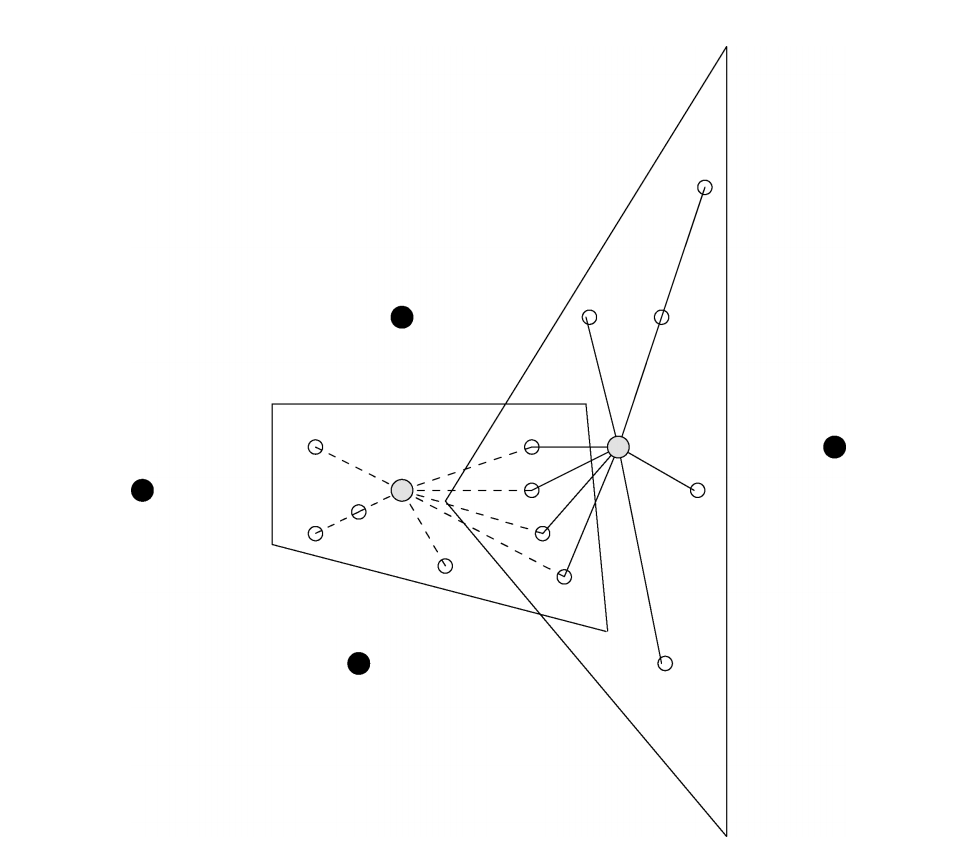
\includegraphics[width=0.8\textwidth]{clusterconstruct.png}
    \caption{Clusters constructed by the modified SSSP algorithm, the figure
             is taken directly from the article\cite{tu}}.
    \label{fig:cluster}
\end{figure}
The clusters are computed by running a modified SSSP algorithm. Due to the
complexity of Thorups SSSP algorithm I will illustrate the modification
on Dijkstra. My implementation used for experiments in later sections also
uses a modified Dijkstra to compute the clusters, so the code is in
agreement with this modification on Dijkstra.

The modification to Dijkstra is in the relaxation step. A normal Dijkstra
relaxes as such
\begin{codebox}
    \Procname{$\proc{relax}(u, v)$}
    \li \If $d(v) > d(u) + \ell(u,v)$
    \li     \Do
            $d(v) = d(u) + \ell(u,v)$
            \End
\end{codebox}
Thorup and Zwick changes this step, so that clusters now are constructed
instead by only including the vertices that are closer to $w$ than to the
$(i+1)$-center.
\begin{codebox}
    \Procname{$\proc{relax\_modified}(u, v)$}
    \li \If $\delta(A_{i+1},v) > d(u) + \ell(u,v)$
    \li     \Do
            $d(v) = d(u) + \ell(u,v)$
            \End
\end{codebox}
After all clusters are constructed the algorithm creates the bunches, as
defined by the algorithm $w \in B(v)$ if and only $v \in C(w)$. The clusters
and the bunches hold the exact same information. The benefit of the bunches
is that the information used by \proc{dist } to find a shortest path can be
stored with the vertex, and thus bunches allow for distance labeling.

The relationship between clusters and bunches is also clear if one takes a
closer look at \autoref{fig:cluster}. E.g if I take a white vertex, that is
a vertex only in $A_0-A_1$, I see that the connected gray vertex should be
part of the bunch, because the gray vertex is closer to the white than to the
black vertex, that is $w \in A_1 - A_2 \,|\, \delta(w,v) < \delta(A_2,v)$.

After the construction of bunches the algorithm terminates and returns the
bunches and witnesses.

\section{Answering shortest distance queries}
The algorithm, \autoref{pseudo:dist}, used to produce estimates from the
constructed data structure is straight forward. The algorithm works by
checking if the vertex $w$ is in the bunch of $v$. If that is not the case $u$
and $v$ are swapped, $i$ is incremented and $w$ is set to $u$'s witness of the
incremented $i$-center. Because $A_{k-1} \in B(v)$ the algorithm will always
terminate.

When $w \in B(v)$ the algorithm returns the estimated distance by reading
$\delta(w,u)$ from the witnesses. The distance $\delta(w,v)$ is read directly
from the bunch $B(v)$.

\begin{figure}[htbp]
\begin{codebox}
    \Procname{$\proc{dist}_{k}(u, v)$}
    \li $w \gets u$
    \li $i \gets 0$ 
    \li \While $w \notin B(v)$
    \li     \Do
                $i \gets i+1$
    \li         $(u,v) \gets (v,u)$
    \li         $w \gets p_{i}(u)$
            \End
    \li \Return $\delta(w,u) + \delta(w,v)$
\end{codebox}
\caption{The distance query algorithm}
\label{pseudo:dist}
\end{figure}

\section{Average stretch of estimates}
From \autoref{eq:stretchinterval} one can see approximate distance oracles
produces results with a stretch guarantee $t$. That is a worst-case multiplicative
factor increase of the distance between a pair of vertices. But this worst case
guarantee may differ substantially from the average multiplicative factor on the
produced distances. For a shortest path query the actual stretch on the distance is
denoted $s$ and is the fraction of the estimated shortest distance over
the exact shortest distance.
\begin{equation}
    s(u,v) = \frac{\hat{\delta}(u,v)}{\delta(u,v)}
\end{equation}
Thus, there will also exist an average actual stretch for a given data structure
\begin{equation}
    \bar{s} = \frac{\sum\limits_{(u,v) \in V \times V} s(u,v) }{|V|^2}
\end{equation}
The article by Thorup and Zwick\cite{tu} does not mention the actual stretch
of the estimates $s$ or the average actual stretch $\bar{s}$. It is my goal to
determine $\bar{s}$ for the graphs used in my experiments, and try to indicate
what values to expect for the classes of graphs used in my experiments.

\newpage
%\chapter{Average stretch of estimates}
From \autoref{eq:stretchinterval} we know approximate distance oracles
produces results with a stretch guarantee. That is a worst-case multiplicative
factor increase of path length between a pair of vertices. But this worst case
guarantee may differ substantial from the average multiplicative factor on the
produces paths. For a single shortest path query the stretch of the result is
denoted $\hat{s}$ and is as the fraction of the exact shortest path.
\begin{equation}
    \hat{s}(u,v) = \frac{\hat{\delta}(u,v)}{\delta(u,v)}
\end{equation}
Thus there will also exists an average such that
\begin{equation}
    \bar{s} = \frac{\sum\limits_{(u,v) \in V \times V} \hat{s}(u,v) }{|V|^2}
\end{equation}

We will try to dertermine $\bar{s}$ through experiments over data from
Stanford Large Network Dataset Collection.

Graphs can have many properties and two graphs may not be suited for using the
algorithm. We have choosen two types of graphs where applications have the need
to answer fast.





\subsection*{Classes of graph we will test}
I have choosen some different areas of graph to see is the results differ.
Roadnet and internet topologies

\begin{description}
  \item[Internet topologies] \hfill
        \begin{description}
        \item[Skitter] \hfill \\
                Internet topology graph. From traceroutes run daily in 2005 -
                \url{http://www.caida.org/tools/measurement/skitter}. From several
                scattered sources to million destinations. 1.7 million nodes, 11
                million edges.

        \item[AS-733] \hfill \\
                The graph of routers comprising the Internet can be organized into
                sub-graphs called Autonomous Systems (AS). Each AS exchanges traffic flows
                with some neighbors (peers). We can construct a communication network of
                who-talks-to- whom from the BGP (Border Gateway Protocol) logs.
        \end{description}
  \item[Road networks] \hfill
        \begin{description}
        \item[California] \hfill \\
                A road network of California. Intersections and endpoints are represented
                by nodes and the roads connecting these intersections or road endpoints are
                represented by undirected edges.

        \item[Texas] \hfill \\
                A road network of Texas. Intersections and endpoints are represented
                by nodes and the roads connecting these intersections or road endpoints are
                represented by undirected edges.

        \item[Pennsylvania] \hfill \\
                A road network of Pennsylvania. Intersections and endpoints are represented
                by nodes and the roads connecting these intersections or road endpoints are
                represented by undirected edges.
    
        \end{description}
\end{description}

The theory of determining the average stretch from experiment is rather
trivial but to sample results data I implemented approximate distance oracles.

%\newpage
\chapter{Implementation}
\label{sec:implementation}
This section discusses key concepts of the approximate distance oracles
implementation made to perform the experiments, and highlights obstacles
and solutions found while developing the implementation. Throughout
the implementation phase, I have tested my solution and benchmarked
my improvements against a graph based on friend lists from Facebook.
The graph has 4039 vertices, 88243 edges, and can be found here
\url{http://snap.stanford.edu/data/egonets-Facebook.html}. This graph I refer
to as the Facebook or test data set.\\\\
All the code is available at \url{https://github.com/brunsgaard/ado}.

\section{Choice of programming language}
The initial attempt to implement approximate distance oracles was done in
Python, but due to extreme memory consumption I reimplemented the algorithm
in C++. \autoref{tab:py_vs_cpp_fb} compares the final C++ implementation of
\proc{prepro} against vanilla Python. C++, as a compiled and heavily optimized
language, has an inherent performance advantage over Python which is an
interpreted language.

Using Google SparseHash\footnote{The Google SparseHash project contains
several hash-map implementations in use at Google, with different performance
characteristics, including an implementation that optimizes for space and
one that optimizes for speed. \url{https://code.google.com/p/sparsehash/}
} 
and multi-threaded processing, the C++ implementation greatly improves both memory
pressure and run times compared against Python.

\begin{table}[htbp]
    \centering
    \begin{tabular}{ l | c | c }
        \toprule
        lang & space & runtime\\
        \midrule
        Python & 118Mb & 39s\\
        C++ & 13Mb & 1s\\
        \bottomrule
    \end{tabular}
    \caption{Performance comparison between C++ and Python implementation,
             when run on \proc{prepro} on facebook test data.}
    \label{tab:py_vs_cpp_fb}
\end{table}

Due to the size of the graphs I use in the experiment, I need low memory
overhead and control over allocation. The memory pressure rapidly increases
with the number of nodes/edges, to the point where a graph with 30000 vertices
and 150000 edges, was barely able to compute with Python on a modern Macbook
pro. The data for which I have to run my experiments is much larger, and thus
the Python implementation was discarded.

\section{Data structures}

The graph is represented as an adjacency list, using a STL\footnote{Standard
Template Library container classes etc for C++, see more at
\url{http://www.sgi.com/tech/stl/stl_introduction.html}} \texttt{vector}
representing the vertices, and a STL \texttt{forward list} (one-way linked
list) for edges. An edge is a \texttt{struct} with just two members, a
memory managed pointer to the vertex and a weight, represented as a double.
\autoref{fig:graph-code-head} show the types and type definition used in the
final solution.

\begin{figure}
\lstset{language=C++}
\begin{lstlisting}
typedef double Weight;
const Weight MaxWeight = std::numeric_limits<double>::infinity();
typedef std::vector<std::shared_ptr<Vertex>> VertexVector;
typedef VertexVector::size_type VertexId;

struct AdjacentNode
{
  std::shared_ptr<Vertex> vertex;
  Weight weight;
  AdjacentNode(std::shared_ptr<Vertex> v, Weight w) : vertex(v), weight(w) {

  }
};

struct Vertex
{
  std::forward_list<AdjacentNode> adjacent;
  VertexId id;
  Vertex(VertexId i) : adjacent(), id(i) {
  }
};
\end{lstlisting}
\caption{graph.h: Code header defining the graph types}
\label{fig:graph-code-head}

\end{figure}

Because all data sets use positive integers as vertex ids, I can use a
\texttt{vector} to represent it, enabling fast constant time lookups. 
However the vector must be initialized in a special way.

First the input data is sequentially scanned to find the largest vertex
id. Then the vector is initialized with nodes from $0$ to the largest
vertex id. I perform an extra vertex allocation for the vertex added, and used
as source when finding the shortest path between $i$-centers and vertices as
mentioned in \autoref{sec:ado:creation}. By allocating it under initialization I
can avoid resizing the vector.

The precision of the \texttt{Weight} is reduced from a double to a float, and
the Vertex ids are reduced from a 64 bit to a 32 bit unsigned integer, when
storing the approximate distance oracle, thus cutting their memory consumption
in half.

\subsection{Preprocessed data}

For the actual data structure I need very memory efficient hash maps, since I 
will be storing a hash map (the cluster) for each node in the graph. Most of
these hash maps will be very sparse, however a few ($w \in A_{k-1}$) will be
dense.

I use Google SparseHash for these hash maps, since it uses an underlying
bitmap improving efficiency with empty buckets. What I gain in memory
efficiency I loose in runtime, so the implementation uses STL
\texttt{unordered\_map} until the very end of preprocessing where it will be
converted to Google's \texttt{sparse\_hash\_map}. \autoref{fig:memcompare}
show the memory consumption on the facebook dataset before and after applying
Google sparse hash to the implementation.

\begin{figure}
    \centering
    \begin{tikzpicture}
        \begin{axis}[
                ybar,
                legend style={at={(0.5,-0.15)},
                    anchor=north,legend columns=-1},
                ylabel=Memory in megabytes,
                symbolic x coords={facebook,enron},
                xtick=data,
                enlarge x limits={abs=60pt},
                bar width=30pt,
                nodes near coords,
                nodes near coords align={vertical},
                ]
            \addplot coordinates {(facebook,14.4) (enron,108.3) };
            \addplot coordinates {(facebook,25.2) (enron,304.9) };
            \legend{Google Sparse Hash,STL unordered\_map}
        \end{axis}
    \end{tikzpicture}
    \caption{Comparison of memory consumption using Google sparse hash and STL
        unordered respectively.}
    \label{fig:memcompare}
\end{figure}

When constructing the data structure, the output data from the modified
Dijkstra is the clusters, so the final step is the creation of bunches,
corresponding to line 11-12 in \autoref{pseudo:prepro}.

This requires the program to keep both clusters and bunches in memory,
effectively doubling the memory usage during the last step. There is no
need for me to convert the clusters into bunches, as I can just access the
information I need in the clusters directly, because I have global access to
all clusters.
This is also mentioned in \autoref{sec:ado:creation}, where I explained that
bunches allows for distance labeling. In my case I have a global state and
can access all information from the clusters directly, thus I do not need
to create bunches. To use the clusters directly, I make a small modification
to the \proc{dist} algorithm in \autoref{pseudo:dist}. The modification is
shown in \autoref{pseudo:dist_mod}, only line 3 has changed.

\begin{figure}[htbp]
\begin{codebox}
    \Procname{$\proc{dist\_mod}_{k}(u, v)$}
    \li $w \gets u$
    \li $i \gets 0$ 
    \li \While $v \notin C(w)$
    \li     \Do
                $i \gets i+1$
    \li         $(u,v) \gets (v,u)$
    \li         $w \gets p_{i}(u)$
            \End
    \li \Return $\delta(w,u) + \delta(w,v)$
\end{codebox}
\caption{The modified distance query algorithm}
\label{pseudo:dist_mod}
\end{figure}

By outputting the clusters to a file I avoid both preprocessing them every
time and keeping them in memory, during processing. Thus the only memory I
need is for a single cluster (or the number of threads calculating clusters),
and a bit for the graph and witnesses. The biggest data set with 1965206
nodes and 2766607 edges uses 1.4 GB memory during cluster creation with
8 threads, well with-in the expectations of modern computers. Before the
clusters were discarded after being written to the output file, memory usage
was in excess of 50 GB, but the program still terminated given enough swap
space (if the bunch creation was left out, otherwise the operating system
killed the process).

For the output files, a custom file format was created for the witnesses and
clusters. To avoid spending cpu cycles on formatting, the data is simply
\emph{reinterpret\_cast}'d to \texttt{unsigned chars}, which means the program
simply treats the memory of an e.g. 4 byte 32-bit integer as 4 bytes of
characters, which can be written directly to a file. For the witnesses this
means that every witness it outputted as a fixed size struct, each containing
the following: $i$-center reference, vertex id, distance and vertex reference
\autoref{tab:witness_ff}. There is no header or delimiter and the number of
bytes used to represent a witness is determined by the underlying types, so if
a type is changed, data structures previously created will be unreadable and
must be re-created.

\begin{table}[htbp]
    \centering
    \begin{tabular}{ | c | c | c | c |}
        \hline
        icenter reference & vertex id & distance & vertex reference.\\
        \hline
        4 bytes (int) & 8 bytes (uint64) & 8 bytes (double) & 8 bytes (int64)\\
        \hline
    \end{tabular}
    \caption{file format of witness, bytes counts are dynamic and/or compiler
             implementation specific}
    \label{tab:witness_ff}
\end{table}

For the clusters I used the built-in Google
SparseHash serializer\footnote{\url{
http://sparsehash.googlecode.com/svn/trunk/doc/sparse\_hash\_map.html\#io}}, 
but combined all clusters into a single file, by adding a header before the
serialized data. This header is 8 bytes (the size of two \texttt{uint32}), and
contains the source vertex id and a 32 bit unsigned integer which represents
the size of the serialized data, after Google SparseHash has serialized it
\autoref{tab:cluster_ff}. Google SparseHash's internal serializing format
includes a built-in delimiter, so multiple hash maps can be stored in same
file, but I still need the custom made size header, because I am reading the
same file from multiple threads \autoref{sec:file_read}.

\begin{table}[htbp]
    \centering
    \begin{tabular}{ | c | c | c |}
        \hline
        vertex id & size n & Google sparse hash \\
        \hline
        4 bytes (uint32) & 4 bytes (uint32) & n bytes (transparent data)\\
        \hline
    \end{tabular}
    \caption{File format of clusters}
    \label{tab:cluster_ff}
\end{table}

\section{Program execution optimization}

In order to optimize execution times, without having to worry too much about
multi-threaded programming, the implementation uses Intel® Threading Building
Blocks (TBB) and C++11 thread features. The only downside to using TBB is the
program is going to be optimized for Intel® CPUs, but recent updates to TBB
includes support for other x86/x86\_64 too.

\subsection{Concurrent preprocessing}\label{sec:multithread_compute}

Since all STL containers are thread safe when one does not mutate them, I can
easily use concurrency to utilize multiple CPU cores while preprocessing the
data. TBB's \texttt{parallel\_for} loop, automatically divides the for loop
work into smaller chunks and spawns the optimal amount of threads, which it
manages. This feature has been used to compute the clusters in parallel.

For writing the data structure to the output file, I need to add thread
safety. This is easily handled by simple mutex lock. Experiments show that
this mutex does not cause lock contention since I am not bottlenecked by
the file output and serialization blocks in the code. If I where, the
serialization could be moved outside the mutex, by serializing to a buffer
first, rather than directly to the file.

\subsection{Concurrent file reading and deserializion}\label{sec:file_read}

The reading and deserialization of Google SparseHash hashmaps is also done
concurrently. For this I use a TBB's \texttt{concurrent\_hash\_map} as the
data structure, because the STL containers are not thread safe for any
non-const methods (mutating).

Each thread \texttt{fopen(3)} the input file in read mode, and reads the
element header. It examines the hash map to check if the vertex id has
already been processed, and if so, skips ahead in the file, corresponding
to the end of the serialized data, which it got from the size header
(\autoref{tab:cluster_ff}). Then it tries to insert the vertex id into
the \texttt{concurrent\_hash\_map}, if it fails then a race condition
occurred and it skips ahead like before. With this style of loading from
the same file, race conditions are very likely to occur, but this is a
non-issue due to the design of \texttt{concurrent\_hash\_map}, this is why
- for my usecase - \texttt{concurrent\_hash\_map} is better than TBB's
\texttt{concurrent\_unordered\_map}, which does not have the same kind of
insert operation.

\newpage
\chapter{Experiments}
\label{sec:experiments}
The goal of the experiments is to determine the average actual stretch of
estimates $\bar{s}$, and also I find it interesting how the actual stretches
are spread in the stretch interval $[1:3]$ on the two different domains of
graphs I have used in my experiments.

The test data consist of five graphs in two domains. Three road networks and
two internet topologies. All graphs are undirected and all edge weights are
$1$. The graphs are from Stanford Large Network Dataset collection\cite{snapnets} and is
described below.
\begin{description}
  \item[Internet topologies] \hfill
        \begin{description}
        \item[Skitter] \hfill \\
                Created from traceroutes run daily in 2005 - From several
                scattered sources to million destinations. 1696415 nodes,
                11095298 edges. Longest shortest path is 25.
        \item[AS-733] \hfill \\
                A communication network of who-talks-to-whom, constructed from
                BGP (Border Gateway Protocol) logs. 6474 nodes, 13895
                edges. Longest shortest path is 9.
        \end{description}
  \item[Road networks] \hfill
        \begin{description}
        \item[California] \hfill \\
                Road network of California. Intersections and endpoints
                are represented by nodes and the roads connecting these
                intersections or road endpoints are represented by undirected
                edges. 1965206 nodes, 2766607 edges. Longest shortest path is
                849.

        \item[Texas] \hfill \\
                Road network of Texas. Intersections and endpoints
                are represented by nodes and the roads connecting these
                intersections or road endpoints are represented by undirected
                edges. 1379917 nodes and 1921660 edges. Longest shortest path
                is 1054.

        \item[Pennsylvania] \hfill \\
                Road network of Pennsylvania. Intersections and endpoints are
                represented by nodes and the roads connecting these
                intersections or road endpoints are represented by undirected
                edges. 1088092 nodes, 1541898 edges. Longest shortest path is
                786.
        \end{description}

\end{description}

I approached the experiments by generating three approximate distance oracle
data structures per graph, and for each of these data structure sample $1000$
vertex pairs, for which the actual stretch has been computed. For each run
the sampled vertex pairs, used to calculate the actual stretch, are the same.
This has been achieved by seeding the random generator with the same seed when
generating the samples. The idea of using the same samples on the three data
structures for a graph, is that only the random selection of $i$-centers in
\proc{prepro} will then effect fluctuation in the actual stretch observed,
thus some noise is removed.

The results are shown by using plots and tables. The plots I use has stretch
on the $y$-axis, and the $x$-axis shows the percentage of observations with a
stretch equal or less to the corresponding value on the $y$-axis.
I find this plot to give a good intuition about the distribution of the
actual stretch values, and at the same time it is easy to read median and
quantiles from the plot. The plot use a different color for results based
on each of the three data structures. The median, mean and max is calculated
on the unified observations for each graph, thus all 3000 observations per
graph are used to calculate these numbers.

All experiments is conducted on a Macbook Pro with 2.3 GHz (i7-4850HQ)
quad-core Intel Core i7 Haswell processor and 16 GB memory. 
Even with all optimizations described in \autoref{sec:implementation}, the
construction of a data structure takes $\sim75$ minutes for the largest of the
graphs in my experiment and consumes $\sim40$ GB storage. But these numbers are
reasonable.

\section{Road networks}
The plot showing the results for the experiment on the Californian road
network is found in \autoref{fig:ca}, and I find that the large majority of
observations has an actual stretch of $1.1$ or below. The median is $1.05$, the
maximum actual stretch observed is $2.41$ and the mean is $1.08$.
\begin{figure}[htbp]
    \centering
    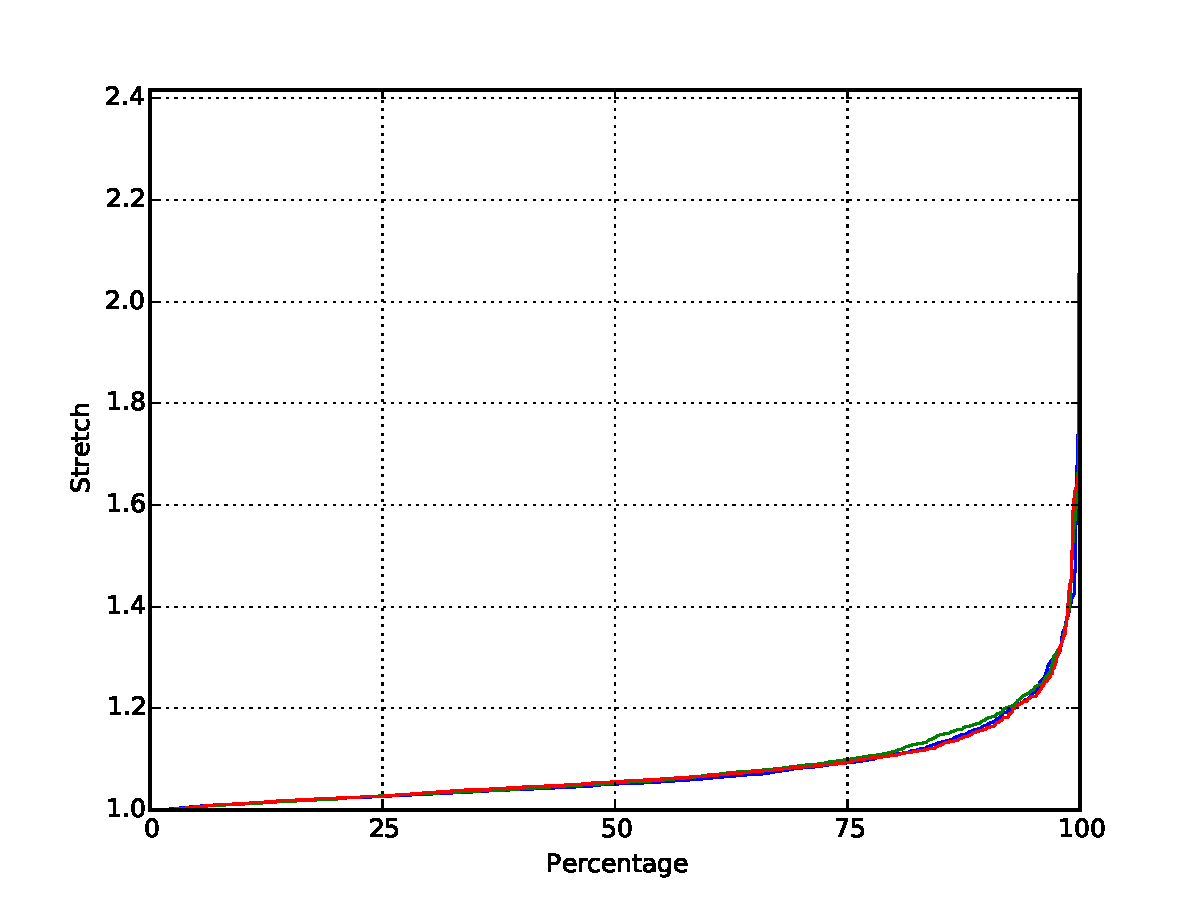
\includegraphics[width=0.8\textwidth]{plots/roadnet_ca.pdf}
    \caption{Actual stretches for California road network, the observations
    from each of the three data structures, has been given different colors.}
    \label{fig:ca}
\end{figure}

For Texas road network the results are very similar. \autoref{fig:tx}
shows how the distribution of the observed actual stretches is more or less
identical to the results found from the graph of California. The experiment
on the road network of Texas shows a median of $1.04$, a mean of $1.06$ and a
maximum actual stretch $2.24$.
\begin{figure}[htbp]
    \centering
    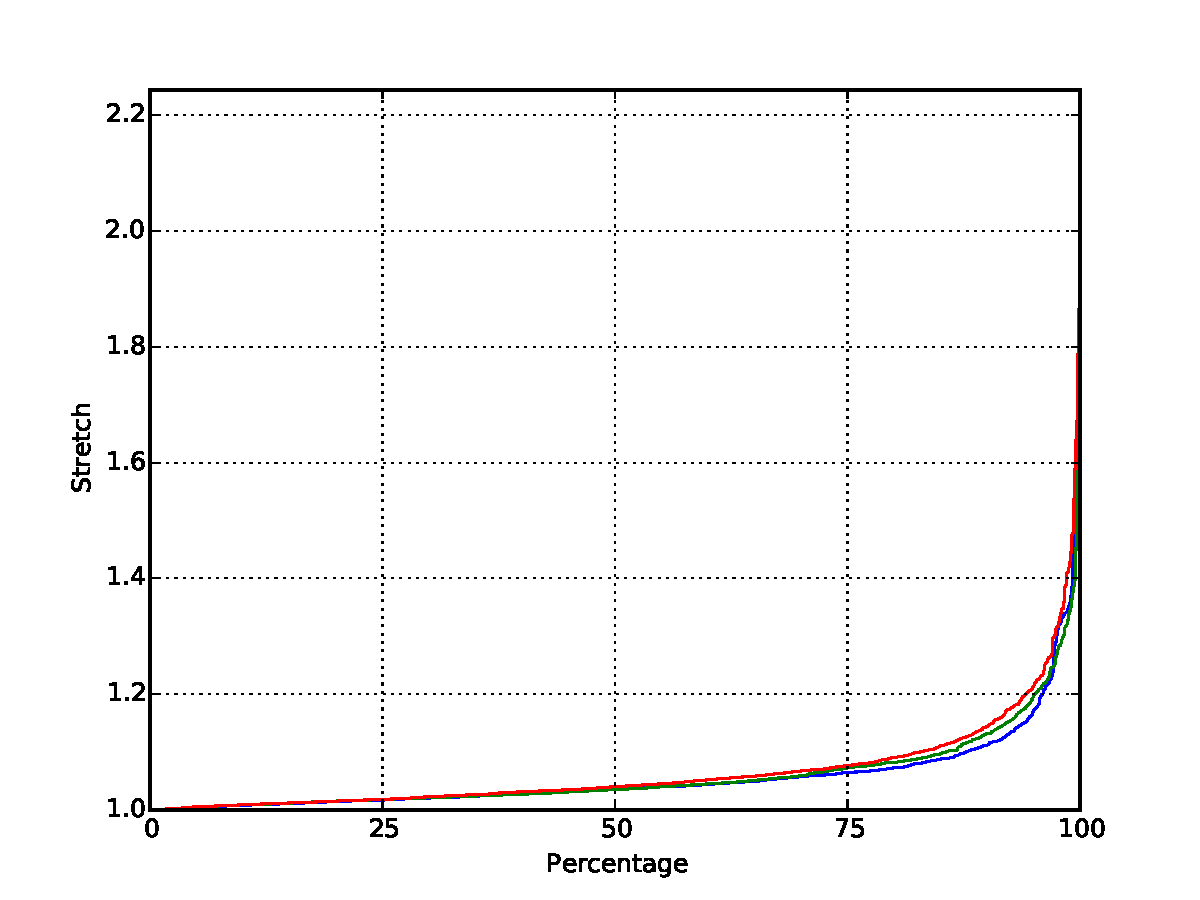
\includegraphics[width=0.8\textwidth]{plots/roadnet_tx.pdf}
    \caption{Actual stretches for Texas road network, the observations
    from each of the three data structures, has been given different colors.}
    \label{fig:tx}
\end{figure}

The graph of Pennsylvania roads, resembles the results from the other road
networks and the experiment returns a median of $1.04$, a mean of $1.07$ and
a maximum observation of $2.33$. \autoref{fig:pa} plots the observations and
it is clear that the shape of the curve and values read from the plot shares
characteristic with the other road networks.

\begin{figure}[htbp]
    \centering
    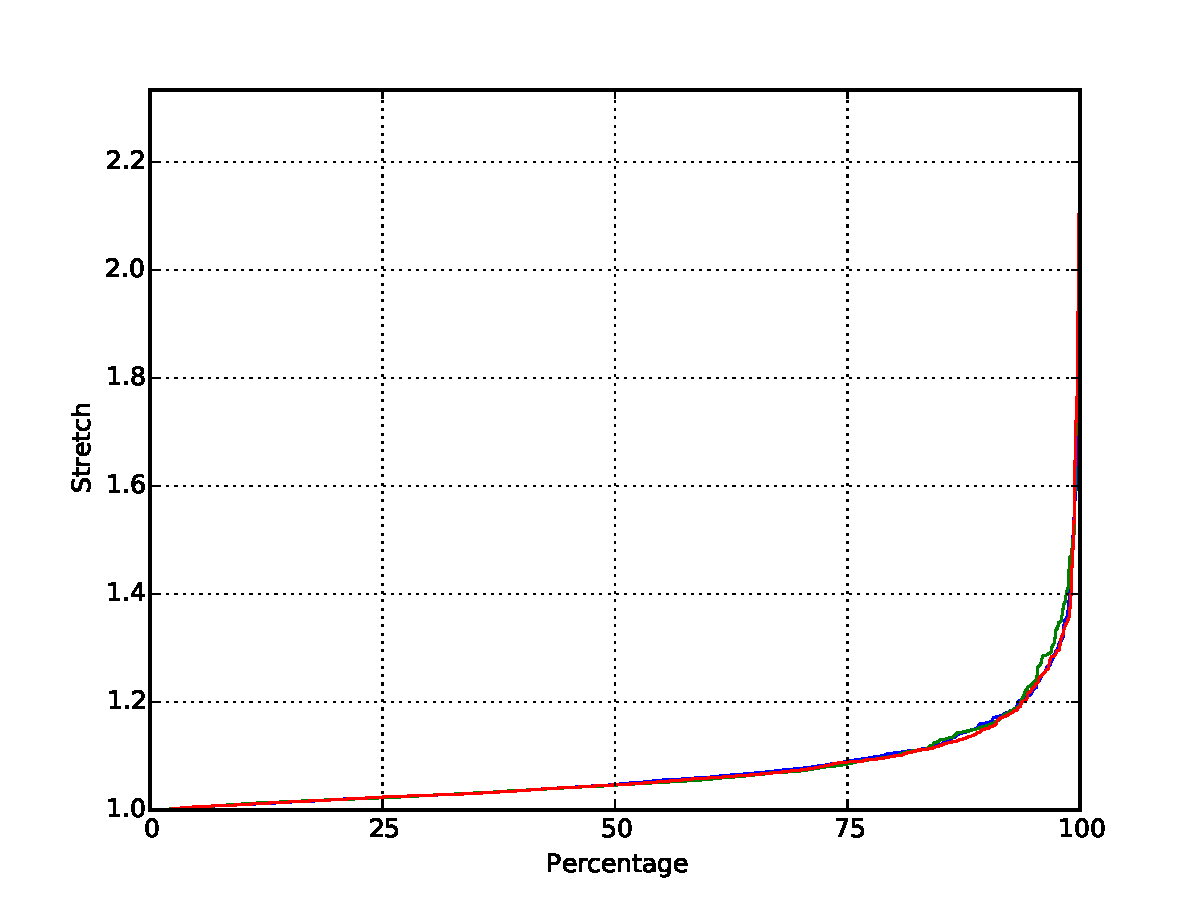
\includegraphics[width=0.8\textwidth]{plots/roadnet_pa.pdf}
    \caption{Actual stretches for Pennsylvania road network, the observations
    from each of the three data structures, has been given different colors.}
    \label{fig:pa}
\end{figure}

The results from running the experiment over the three road network data sets,
indicate that the actual stretches and actual stretch distribution in this
graph domain is very similar and I find the low stretch and low deviations very
impressive. \autoref{tab:roadmap} sums up the results for median, mean, and max.
\begin{table}[htbp]
    \centering
    \begin{tabular}{ l | c | c | c }
        \toprule
             & CA & TX & PA \\
        \midrule
        Median & 1.05 & 1.04 & 1.04 \\
        Max. & 2.41 & 2.24 & 2.33 \\
        \midrule
        Mean. & 1.08 & 1.06 & 1.07 \\
    \end{tabular}
    \caption{Median, maximum and mean for road networks}
    \label{tab:roadmap}
\end{table}
\clearpage

\section{Internet topologies}

For the Skitter topology I find a median of $1.40$ which is substantially
higher than medians found in the road networks. The mean follows the
median and is found to be $1.40$. The maximum actual stretch observed is
$3.0$, which is equal to worst-case. A plot for the experiment is found in
\autoref{fig:skitter}.
\begin{figure}[htbp]
    \centering
    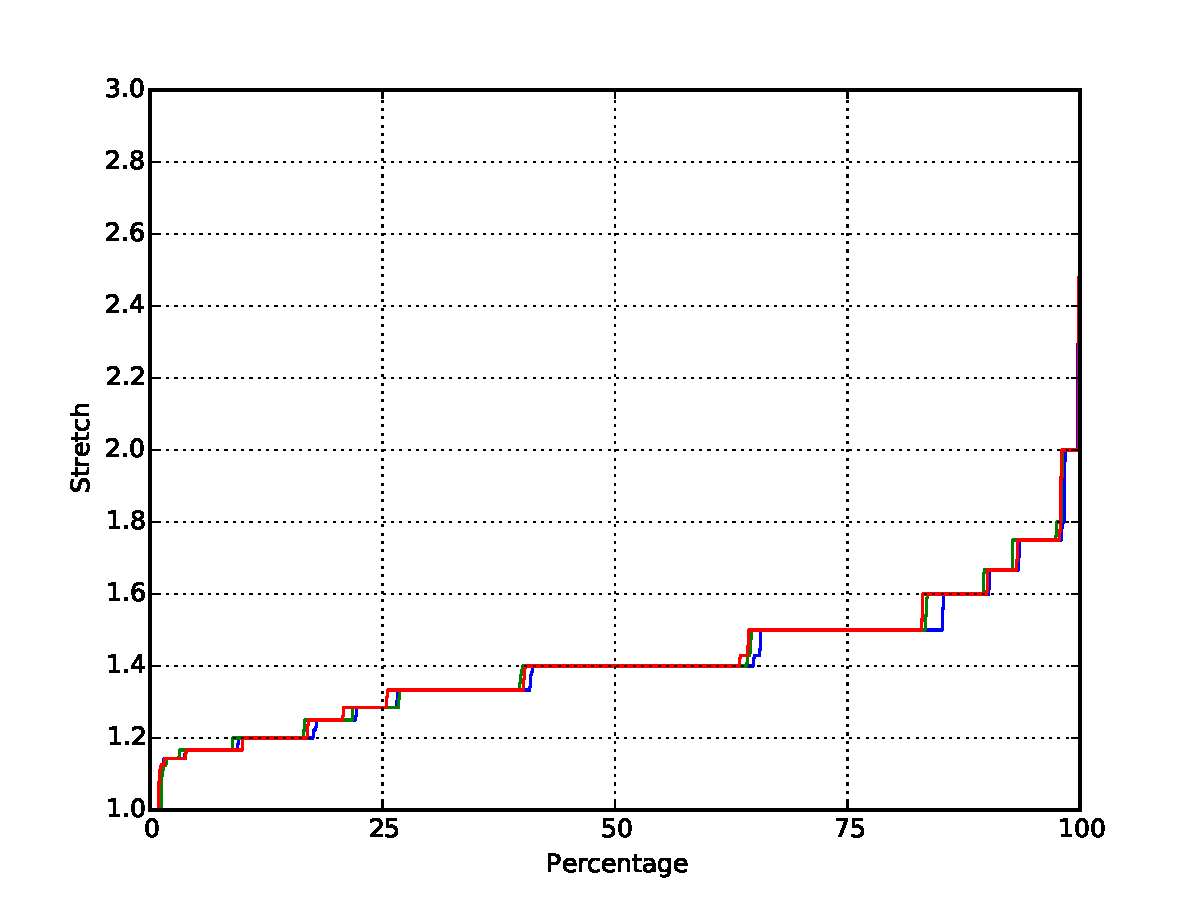
\includegraphics[width=0.8\textwidth]{plots/as_skitter.pdf}
    \caption{Actual stretches for Skitter internet topology, the observations
    from each of the three data structures, has been given different colors.}
    \label{fig:skitter}
\end{figure}

For AS-733 the median is even higher with a value of $1.50$. Also the mean
is higher than we have seen in the other experiments. The mean is $1.56$ and
the maximum actual stretch is again $3.0$. The plot for the stretches of
AS-733 is shown in \autoref{fig:as733}.
\begin{figure}[htbp]
    \centering
    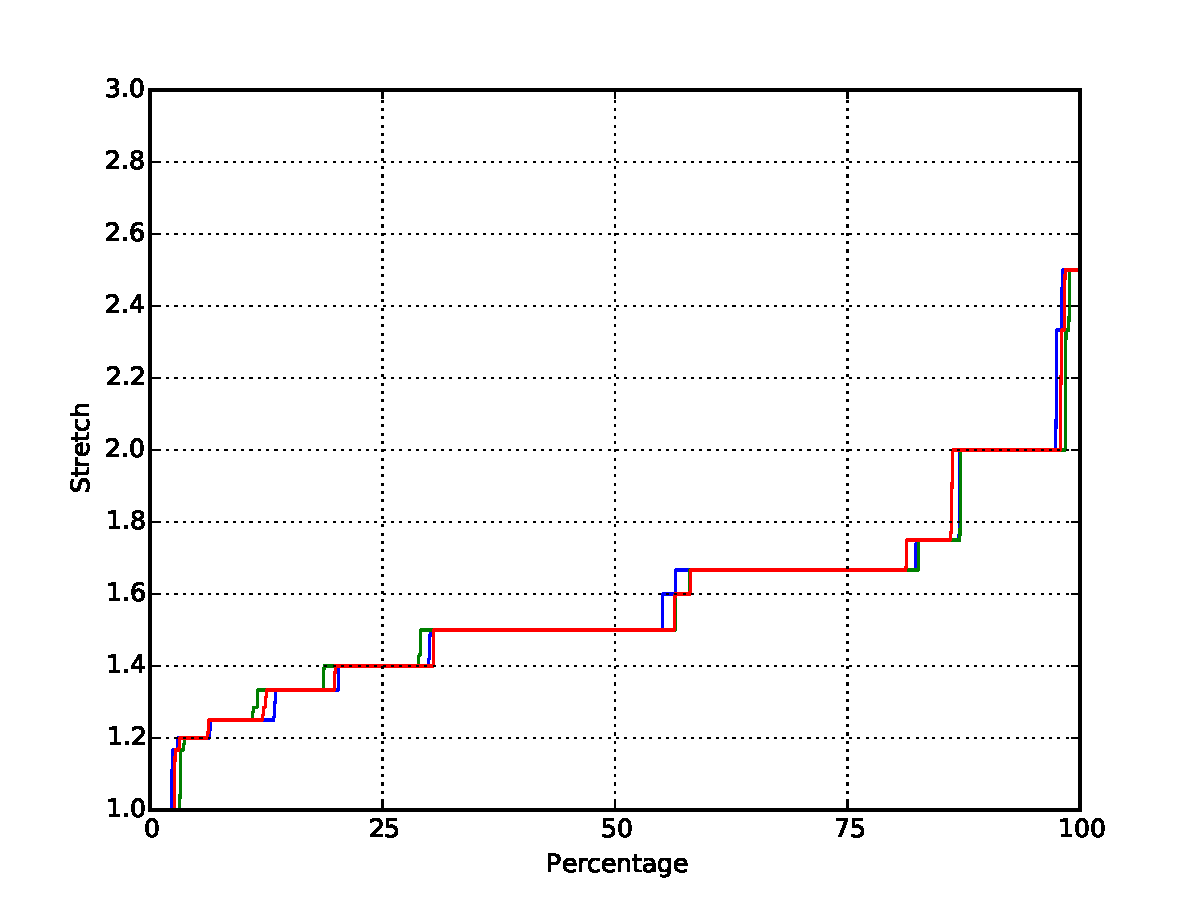
\includegraphics[width=0.8\textwidth]{plots/as_733.pdf}
    \caption{Actual stretches for AS-733 internet topology, the observations
    from each of the three data structures, has been given different colors.}
    \label{fig:as733}
\end{figure}

Again I see similarities between the graphs in this domain.
Even though the graphs differ a lot in size, the average actual stretches is
very close to each other. Also the plots looks very similar, which indicates that
the distribution of the actual stretches is similar for these internet topologies.
\autoref{tab:internettopo} sums up the median, maximum and mean for Skitter
and AS-733.

\begin{table}[htbp]
    \centering
    \begin{tabular}{ l | c | c }
        \toprule
             & Skitter & AS-733 \\
        \midrule
        Median & 1.40 & 1.50 \\
        Max. & 3.0 & 3.0 \\
        \midrule
        Mean. & 1.40 & 1.56 \\
    \end{tabular}
    \caption{Median, maximum and mean for Skitter and AS-733}
    \label{tab:internettopo}
\end{table}

\newpage
\chapter{Conclusion}
\label{sec:conclusion}

Based on this report I can conclude that making an efficient implementation
of approximate distance oracles, capable of handling data sets with millions
of nodes, requires the use of heavily performance optimized language, memory
efficient data structures and concurrent programming, where the algorithm
allows for it.

In this report I have provided empirical data that suggests the average actual
stretch of $k=2$ approximate distance oracles data structures is considerably
lower than the worst case stretch of $3$. I have tested the actual stretch
on two internet topologies and three road network and the maximum value for
$\bar{s}$ I have been able to produce is $1.56$. The internet topologies
domain has a combined mean of $1.48$ and the road networks $1.07$, which I
find to be a fine overall result.

My experiments also suggest that the average actual stretch produced by
approximate distance oracles on graphs within the same domain is very similar.
Also the distribution of the graph stretches seems related for the results
generated within the domain.

For graphs in the domain of internet topologies, I have observed that both
data sets used in the experiments produce results in the same range and their
distribution of the produced stretches are similar. So I find that $\bar{s}
\approx 1.5$ is a reasonable indicator for the average actual stretch found in
internet topologies.

Furthermore, the experiments run over road networks for California, Texas and
Pennsylvania produce exciting results. Not only are the distributions and
averages of the actual stretches produced from the created data structures
more or less identical. The mean value is found to be approximately $1.1$,
which I find impressive. This indicates that graphs from this domain possess
similar properties that makes approximate distance oracles produce very good
estimates.


\newpage
\bibliographystyle{amsplain}
\bibliography{../../references}


\end{document}
